\section{Confinement Modes}
\begin{frame} {Confinement Modes}
    \begin{itemize}
        \item \textbf{Ohmically heated plasmas}:
              \[ \tau_E = 0.07(n/10^{20})aR^2q\]
              Confinement increases as density increases.
        \item \textbf{L-mode}:
              \[ \tau_E^{ITER89-P} = 0.048\frac{I^{0.85}R^{1.2}a^{0.3}\kappa^{0.5}(n/10^{20})^{0.1}B^{0.2}A^{0.5}}{P^{0.5}} \]
              Confinement drops and heating power $P$ increases.
        \item \textbf{H-mode}:
              \[ \tau_{Th}^{ITER H93-P} = 0.053\frac{I^{1.06}R^{1.9}a^{-0.11}\kappa^{0.66}(n/10^{20})^{0.17}B^{0.32}A^{0.41}}{P^{0.67}} \]
              $\tau_{Th}$ refers to confinement time for the thermal part of the plasma energy. It is valid without edge localized modes (ELMs).
    \end{itemize}
\end{frame}

\begin{frame} {H-modes}
    \begin{itemize}
        \item H-mode has good confinement.
        \item At the edge, shape density gradient is steep.
        \item Transport barrier at the edge is developed.
    \end{itemize}
    \begin{figure}
        \centering
        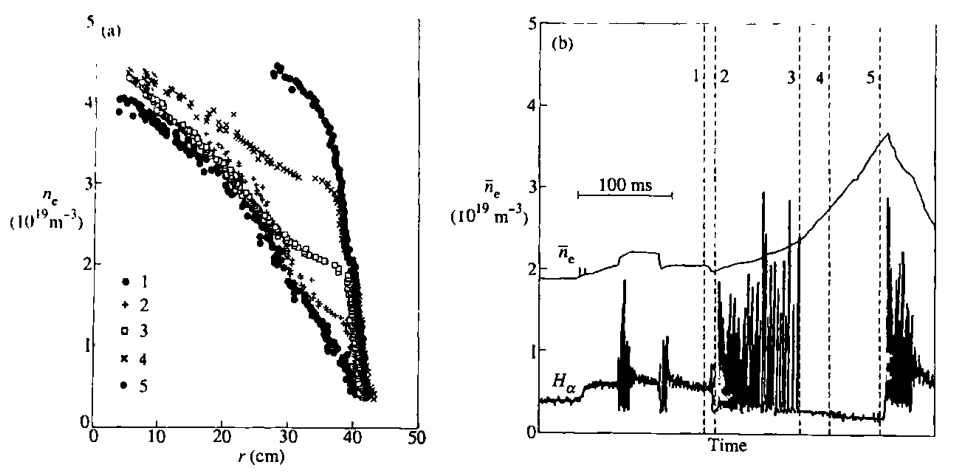
\includegraphics[width=0.7\textwidth]{figures/h-mode.png}
        \caption{Sequence of density profiles measured on ASDEX through and following an L-H transition. The profiles in (a) are at the times shown in (b), which gives the time dependence of $\bar{n}_e$ and the $H_\alpha$ signal.}
        \label{fig:h-mode}
    \end{figure}
\end{frame}

\begin{frame} {Internal Transport Barriers}
    \begin{figure}
        \centering
        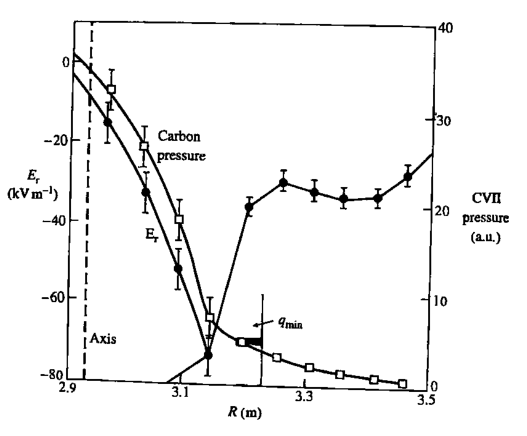
\includegraphics[width=0.5\textwidth]{figures/internal-transport-barrier.png}
        \caption{Radial electric field and carbon pressure profiles in an ERS discharge in TFTR. Fluctuations and turbulent fluxes are reduced inside the transport barrier near the minimum in $q$. Correspondingly, the carbon pressure profile has a stepper gradient in this region. The transport barrier is associated with a rapidly varying profile of $E_r$.}
        \label{fig:internal-transport-barrier}
    \end{figure}
\end{frame}
